
\documentclass[border=10pt, 12pt]{standalone}
\usepackage[svgnames]{xcolor}
\usepackage{amsmath}
\usepackage{pgfplots}
\pgfplotsset{compat=newest}
\usepackage[sfdefault]{FiraSans}
\usepackage{FiraMono}
\renewcommand*\familydefault{\sfdefault}
\begin{document}
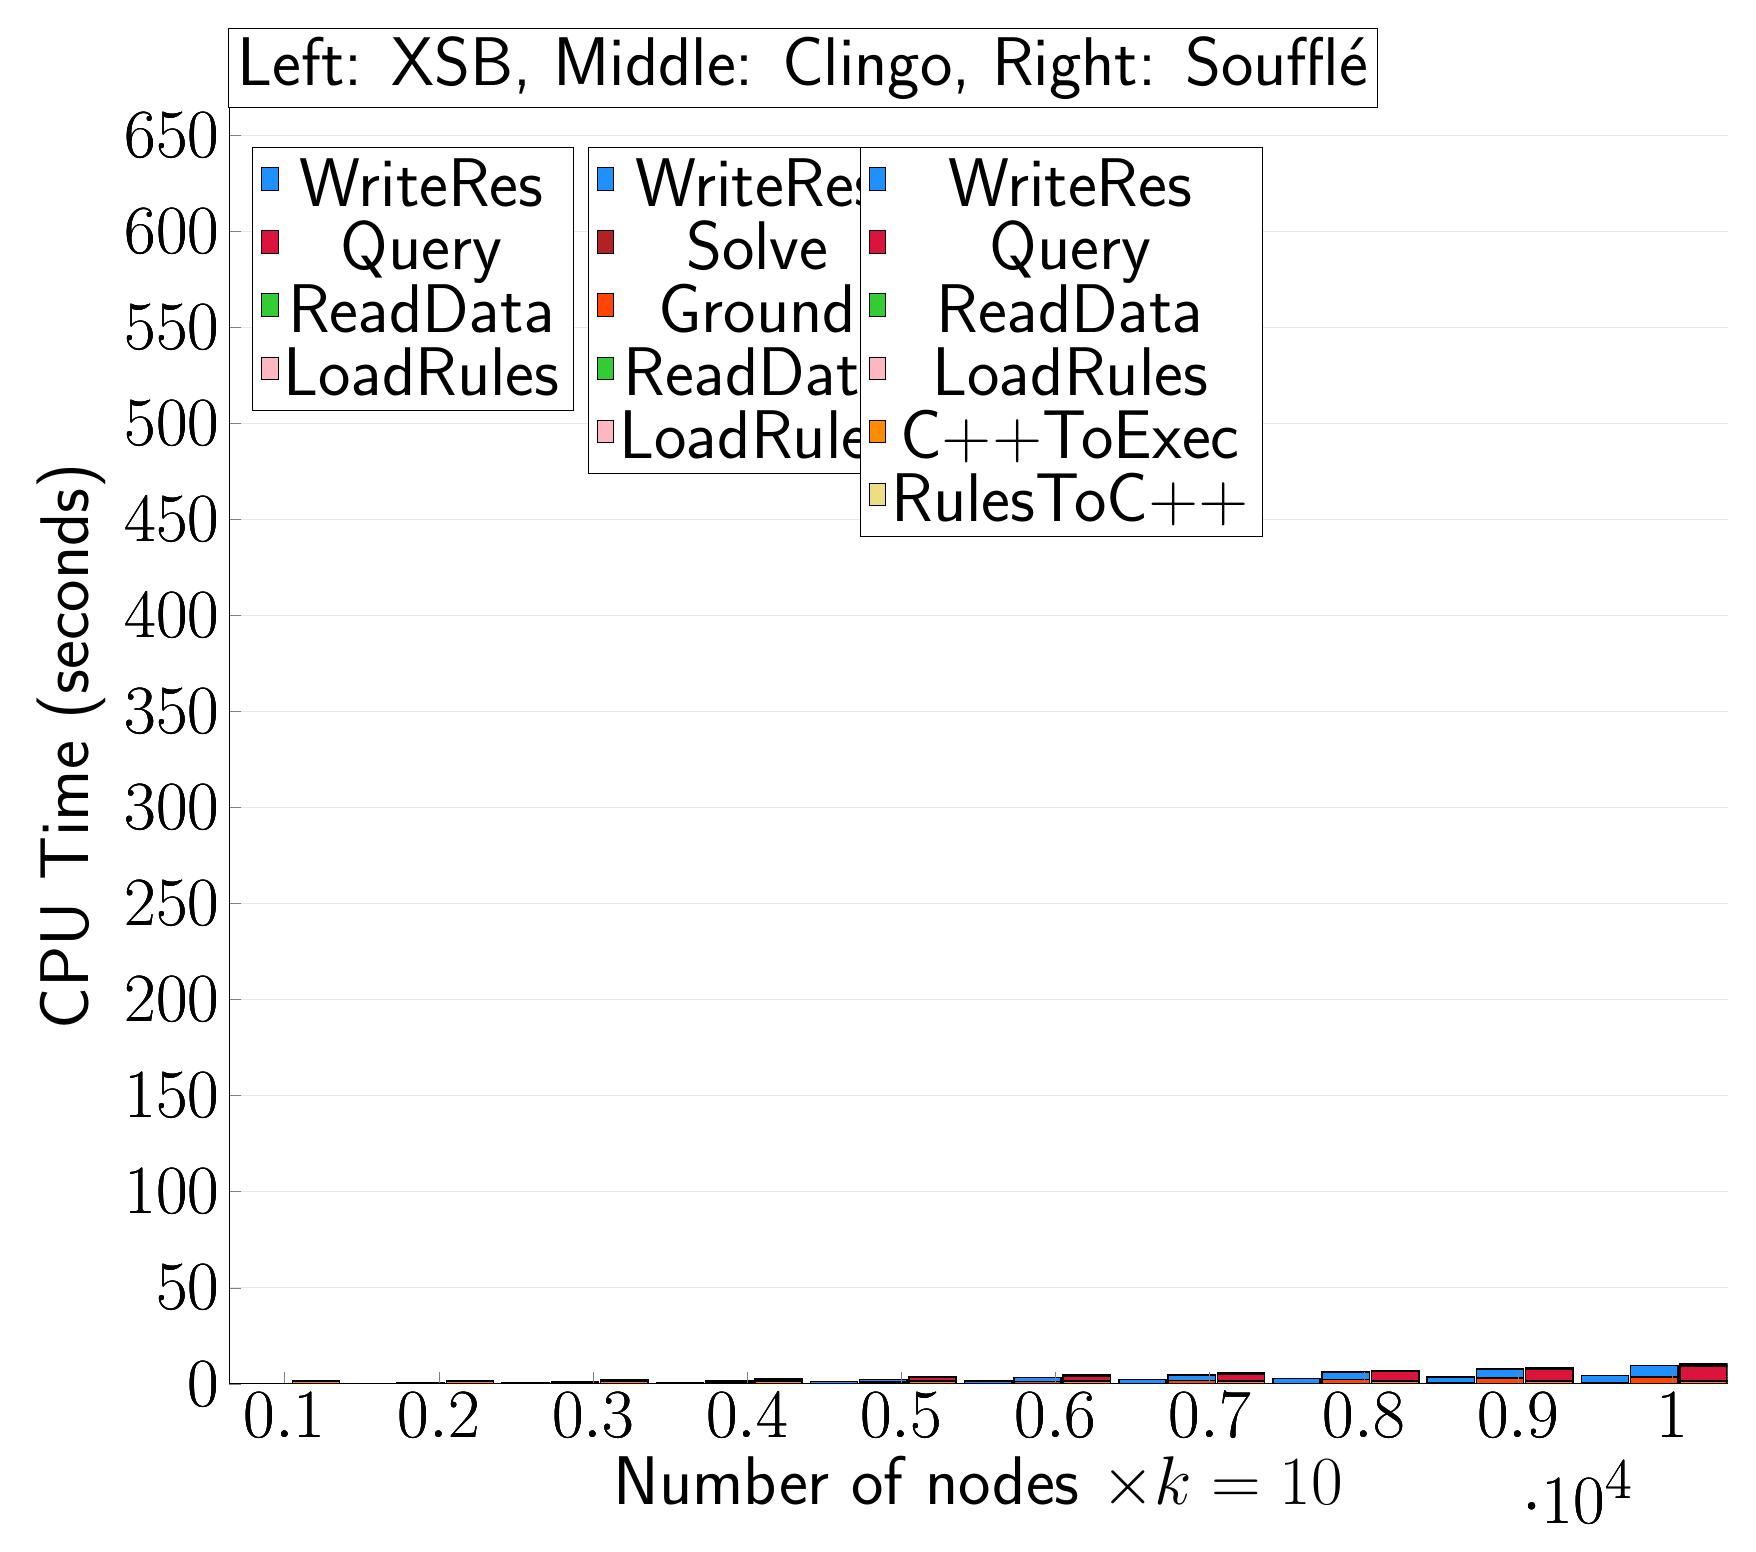
\begin{tikzpicture}
                        \begin{axis}[bar shift=-24.3pt, 
   ybar stacked,
   width=1.7\textwidth,
   bar width=0.6cm,
   ymajorgrids, tick align=inside,
   major grid style={draw=gray!20},
   xtick=data,
   ymin=0, ymax=664.059,
   axis x line*=bottom,
   axis y line*=left,
   enlarge x limits=0.04,
   legend style={
       at={(0.23, 0.97)},
       anchor=north east,
       legend columns=1,
       font=\Huge,
   },
   ylabel={CPU Time (seconds)},
   xlabel={Number of nodes $\times k=10$},
   label style={font=\Huge},
   tick label style={font=\Huge},
]
\addlegendimage{fill=DodgerBlue, draw=black, line width=0.2pt}
\addlegendentry{WriteRes}
\addlegendimage{fill=Crimson, draw=black, line width=0.2pt}
\addlegendentry{Query}
\addlegendimage{fill=LimeGreen, draw=black, line width=0.2pt}
\addlegendentry{ReadData}
\addlegendimage{fill=LightPink, draw=black, line width=0.2pt}
\addlegendentry{LoadRules}
\addplot +[fill=LightPink, draw=black, line width=0.55pt] coordinates {
(1000, 0.0005557999999999993)
(2000, 0.0005502)
(3000, 0.0005507999999999998)
(4000, 0.0005552000000000003)
(5000, 0.0005551999999999996)
(6000, 0.0005636)
(7000, 0.0005798000000000002)
(8000, 0.0005587999999999997)
(9000, 0.0005642)
(10000, 0.0005578000000000004)
};
\addplot +[fill=LimeGreen, draw=black, line width=0.55pt] coordinates {
(1000, 0.0009046000000000004)
(2000, 0.0017323999999999998)
(3000, 0.0025754)
(4000, 0.0033852)
(5000, 0.004215399999999999)
(6000, 0.005068399999999999)
(7000, 0.0059126000000000005)
(8000, 0.0066549999999999995)
(9000, 0.007484)
(10000, 0.0083582)
};
\addplot +[fill=Crimson, draw=black, line width=0.55pt] coordinates {
(1000, 0.0041836)
(2000, 0.0164796)
(3000, 0.036288)
(4000, 0.0647062)
(5000, 0.09865600000000001)
(6000, 0.1414584)
(7000, 0.19492939999999997)
(8000, 0.25188260000000007)
(9000, 0.3158156)
(10000, 0.3937694)
};
\addplot +[fill=DodgerBlue, draw=black, line width=0.55pt] coordinates {
(1000, 0.04018000000000001)
(2000, 0.1600954)
(3000, 0.3613)
(4000, 0.640775)
(5000, 0.9989397999999999)
(6000, 1.4400334)
(7000, 1.9694023999999999)
(8000, 2.5503692)
(9000, 3.2279849999999994)
(10000, 4.0077868)
};
\end{axis}

\begin{axis}[bar shift=-6.5pt, 
   ybar stacked,
   width=1.7\textwidth,
   bar width=0.6cm,
   ymajorgrids, tick align=inside,
   major grid style={draw=none},
   xtick=data,
   ymin=0, ymax=664.059,
   axis x line*=none,
   axis y line*=none,
   enlarge x limits=0.04,
   legend style={
       at={(0.454, 0.97)},
       anchor=north east,
       legend columns=1,
       font=\Huge,
   },
   label style={font=\Huge},
   tick label style={font=\Huge},
]
\addlegendimage{fill=DodgerBlue, draw=black, line width=0.2pt}
\addlegendentry{WriteRes}
\addlegendimage{fill=FireBrick, draw=black, line width=0.2pt}
\addlegendentry{Solve}
\addlegendimage{fill=OrangeRed, draw=black, line width=0.2pt}
\addlegendentry{Ground}
\addlegendimage{fill=LimeGreen, draw=black, line width=0.2pt}
\addlegendentry{ReadData}
\addlegendimage{fill=LightPink, draw=black, line width=0.2pt}
\addlegendentry{LoadRules}
\addplot +[fill=LightPink, draw=black, line width=0.55pt] coordinates {
(1000, 0.0)
(2000, 0.0)
(3000, 0.0)
(4000, 0.0)
(5000, 0.0)
(6000, 0.0)
(7000, 0.0)
(8000, 0.0)
(9000, 0.0)
(10000, 0.0)
};
\addplot +[fill=LimeGreen, draw=black, line width=0.55pt] coordinates {
(1000, 0.0)
(2000, 0.0)
(3000, 0.0)
(4000, 0.008000000000000007)
(5000, 0.010000000000000009)
(6000, 0.010000000000000009)
(7000, 0.010000000000000009)
(8000, 0.010000000000000009)
(9000, 0.020000000000000018)
(10000, 0.020000000000000018)
};
\addplot +[fill=OrangeRed, draw=black, line width=0.55pt] coordinates {
(1000, 0.030000000000000027)
(2000, 0.11599999999999999)
(3000, 0.266)
(4000, 0.4779999999999999)
(5000, 0.784)
(6000, 1.1620000000000001)
(7000, 1.616)
(8000, 2.13)
(9000, 2.8080000000000003)
(10000, 3.418)
};
\addplot +[fill=FireBrick, draw=black, line width=0.55pt] coordinates {
(1000, 0.0)
(2000, 0.014000000000000009)
(3000, 0.02200000000000002)
(4000, 0.054000000000000034)
(5000, 0.08400000000000007)
(6000, 0.12400000000000011)
(7000, 0.16799999999999993)
(8000, 0.21600000000000003)
(9000, 0.26)
(10000, 0.3580000000000002)
};
\addplot +[fill=DodgerBlue, draw=black, line width=0.55pt] coordinates {
(1000, 0.06)
(2000, 0.22599999999999992)
(3000, 0.5360000000000001)
(4000, 0.9159999999999998)
(5000, 1.456)
(6000, 2.088)
(7000, 2.8040000000000007)
(8000, 3.7620000000000005)
(9000, 4.6259999999999994)
(10000, 5.770000000000001)
};
\end{axis}

\begin{axis}[bar shift=11.3pt, 
   ybar stacked,
   width=1.7\textwidth,
   bar width=0.6cm,
   ymajorgrids, tick align=inside,
   major grid style={draw=none},
   xtick=data,
   ymin=0, ymax=664.059,
   axis x line*=none,
   axis y line*=none,
   enlarge x limits=0.04,
   legend style={
       at={(0.69, 0.97)},
       anchor=north east,
       legend columns=1,
       font=\Huge,
   },
   label style={font=\Huge},
   tick label style={font=\Huge},
]
\addlegendimage{fill=DodgerBlue, draw=black, line width=0.2pt}
\addlegendentry{WriteRes}
\addlegendimage{fill=Crimson, draw=black, line width=0.2pt}
\addlegendentry{Query}
\addlegendimage{fill=LimeGreen, draw=black, line width=0.2pt}
\addlegendentry{ReadData}
\addlegendimage{fill=LightPink, draw=black, line width=0.2pt}
\addlegendentry{LoadRules}
\addlegendimage{fill=DarkOrange, draw=black, line width=0.2pt}
\addlegendentry{C++ToExec}
\addlegendimage{fill=LightGoldenrod, draw=black, line width=0.2pt}
\addlegendentry{RulesToC++}
\addplot +[fill=LightGoldenrod, draw=black, line width=0.55pt] coordinates {
(1000, 0.0020000000000000005)
(2000, 0.0)
(3000, 0.008000000000000002)
(4000, 0.004000000000000001)
(5000, 0.006000000000000001)
(6000, 0.0020000000000000005)
(7000, 0.004000000000000001)
(8000, 0.003999999999999997)
(9000, 0.0020000000000000005)
(10000, 0.004000000000000001)
};
\addplot +[fill=DarkOrange, draw=black, line width=0.55pt] coordinates {
(1000, 1.464)
(2000, 1.4700000000000002)
(3000, 1.464)
(4000, 1.464)
(5000, 1.464)
(6000, 1.464)
(7000, 1.468)
(8000, 1.4740000000000002)
(9000, 1.47)
(10000, 1.4739999999999998)
};
\addplot +[fill=LightPink, draw=black, line width=0.55pt] coordinates {
(1000, 0.00016380000000000002)
(2000, 0.00015539999999999998)
(3000, 0.0001542)
(4000, 0.0001516)
(5000, 0.0001572)
(6000, 0.0001576)
(7000, 0.00015600000000000002)
(8000, 0.0001776)
(9000, 0.0001626)
(10000, 0.00016820000000000002)
};
\addplot +[fill=LimeGreen, draw=black, line width=0.55pt] coordinates {
(1000, 0.0039168)
(2000, 0.0074026)
(3000, 0.0103216)
(4000, 0.013134799999999999)
(5000, 0.0147482)
(6000, 0.017763400000000002)
(7000, 0.0203146)
(8000, 0.0219982)
(9000, 0.0223614)
(10000, 0.024902600000000004)
};
\addplot +[fill=Crimson, draw=black, line width=0.55pt] coordinates {
(1000, 0.0798616)
(2000, 0.2782822)
(3000, 0.6315489999999999)
(4000, 1.1465020000000001)
(5000, 1.811404)
(6000, 2.6391560000000003)
(7000, 3.6447720000000006)
(8000, 4.8037019999999995)
(9000, 6.141988)
(10000, 7.659197999999999)
};
\addplot +[fill=DodgerBlue, draw=black, line width=0.55pt] coordinates {
(1000, 0.0109124)
(2000, 0.0432664)
(3000, 0.098179)
(4000, 0.17308759999999998)
(5000, 0.270248)
(6000, 0.39185800000000004)
(7000, 0.526502)
(8000, 0.6883712)
(9000, 0.8682051999999999)
(10000, 1.064892)
};
\end{axis}


\node[anchor=south, draw, fill=white] at (rel axis cs:0.42,1) {\Huge Left: XSB, Middle: Clingo, Right: Soufflé};
\end{tikzpicture}
\end{document}
                    